\documentclass[11pt,a4paper]{article}

\usepackage[utf8]{inputenc} 
\usepackage[T1]{fontenc} 
\usepackage{lmodern}
\usepackage[margin=2cm]{geometry}
\usepackage[german]{babel}
\usepackage{amsmath} 
\usepackage{graphicx} 
\usepackage{booktabs}
\usepackage{hyperref}
\usepackage{mathtools}
\hypersetup{
    colorlinks,
    citecolor=red,
    filecolor=black,
    linkcolor=black!20!blue!90!,
    urlcolor=black} 
\usepackage{nicefrac}
\usepackage[table]{xcolor}
\usepackage{tocloft}

\setlength{\parindent}{0pt}
\setlength{\parskip}{1ex plus 0.5ex minus 0.5ex}

\definecolor{incolor}{rgb}{0.0, 0.0, 0.5}

\hbadness=99999

\newcommand{\refpy}[1]{Siehe Anhang: \textit{Rechnungen in Python} (\texttt{{\color{incolor}In [{\color{incolor}#1}]}})}
\newcommand\dif{\mathop{}\!\mathrm{d}}
\newcommand\mean{\begin{equation}
\frac{\sum_{i=1}^n I_{V_i}}{n}\label{mean}
\end{equation}}
\newcommand\meanstd{\begin{equation}
s_x=\sqrt{\frac{1}{n-1}\sum_{i=1}^n(x_i-\overline{x})^2}\label{meanstd}
\end{equation}}
\newcommand\prodquo{\begin{equation}\left\vert\frac{\Delta z}{z}\right\vert=\sqrt{\left(a\frac{\Delta x}{x}\right)^2+\left(b\frac{\Delta y}{y}\right)^2+\ldots}\textrm{ f\"ur }z=x^a\ y^b\ldots\end{equation}}
\newcommand\tfnc{\begin{equation}
\frac{\vert x-y_0\vert}{u_x}
\end{equation}}
\newcommand{\halftime}[4]{\begin{figure}[h]
\begin{minipage}{.#1\textwidth}#3\end{minipage}\begin{minipage}{.#2\textwidth}
\centering
#4\end{minipage}
\end{figure}}
\renewcommand{\vec}{\boldsymbol}

\begin{document}

{
\centering 
\large 
Physiklabor für Anf\"anger*innen \\
Ferienpraktikum im Sommersemester 2018 \\[4mm]
\textbf{\LARGE 
Versuch 06: Elastizitätskonstante
} \\[3mm]
(durchgef\"uhrt am 24.09.2018 bei Julia Müller) \\
Andréz Gockel, Patrick M\"unnich\\
\today \\[10mm]
}

\vspace{50pt}
\tableofcontents
\vspace{22pt}
\listoftables
\vspace{22pt}
\listoffigures
\pagebreak
\phantom{lol}
\thispagestyle{empty}
\pagebreak


\section{Ziel des Versuchs}

Das Ziel des Versuchs ist es, den Elastizit\"atsmodul von drei unterschiedlichen isotropen Festk\"orpern mittels Biegung zu ermitteln. Au\ss erdem soll die Abh\"angigkeit der Biegung eines Stabes mit rechteckigen Querschnitt vom Material, der Ausrichtung und der L\"ange untersucht werden.

\section{Versuch}

\subsection{Theorie}

Wird eine (nicht all zu gro\ss e) Kraft $F$ auf einen elastischen Festk\"orper ausge\"ubt, so f\"uhrt dies zu einer L\"angen\"anderung $\Delta l$. F\"ur hinreichend kleiner Kr\"afte ist die L\"angen\"anderung proportional zur angreifenden Kraft. Den Kehrwert dieser Proportionalit\"atskonstante wird als Elastizit\"atsmodul $E$ bezeichnet (\textit{Hooke}'sches Gesetz):

\begin{equation}
\frac{\Delta l}{l}=\frac{F}{EA}=\frac{\sigma}{E}\label{eq:elast}
\end{equation}

Wie in Abbildung \ref{Abb:1} zu erkennen, f\"uhrt die Biegung eines Balkens zu Stauchung und Streckung oberhalb und unterhalb der sog. \textit{neutralen Faser}.

\begin{figure}[h]
\centering
\fbox{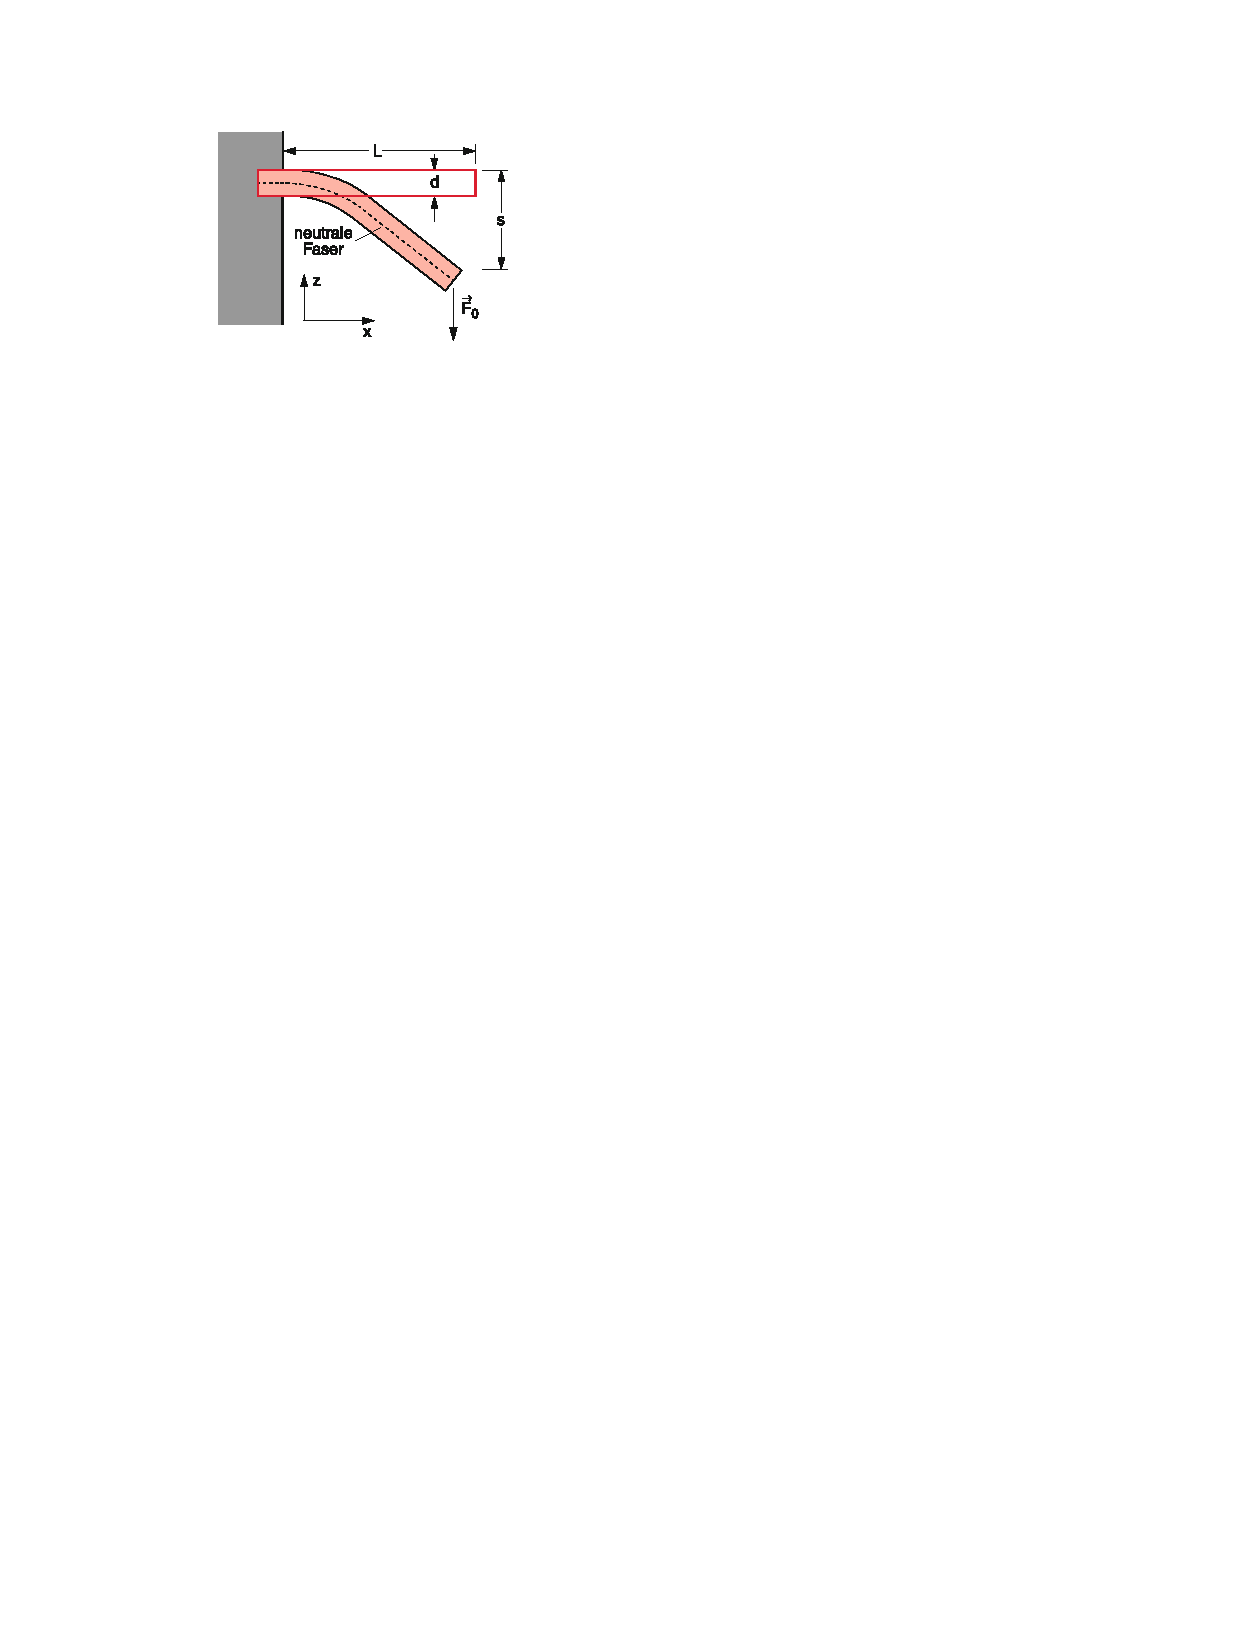
\includegraphics[width=0.8\textwidth]{neutraleFaser.pdf}}
\renewcommand\thefigure{B1}
\caption[Biegung eines Stabes unter Einfluss einer Kraft $F_0$ mit neutraler Faser]{Biegung eines Stabes unter Einfluss einer Kraft $F_0$ mit neutraler Faser \cite{Demtr\"oder}}
\label{Abb:1}
\end{figure}

\pagebreak

Nach dem \textit{Hooke}'schen Gesetz ist diese Biegung/Stauchung f\"ur kleine Gewichte proportional zur angreifenden Kraft. F\"ur einen Balken, der an beiden Enden unterst\"utzt wird (Abbildung \ref{Abb:2}), ergibt sich

\begin{equation}
s\mathrel{:\mkern-0.25mu=} z(x=\nicefrac{l}{2})=\frac{1}{E}\frac{l^3}{4h^3b}F\label{eq:biegp}
\end{equation}

\begin{figure}[h]
\centering
\fbox{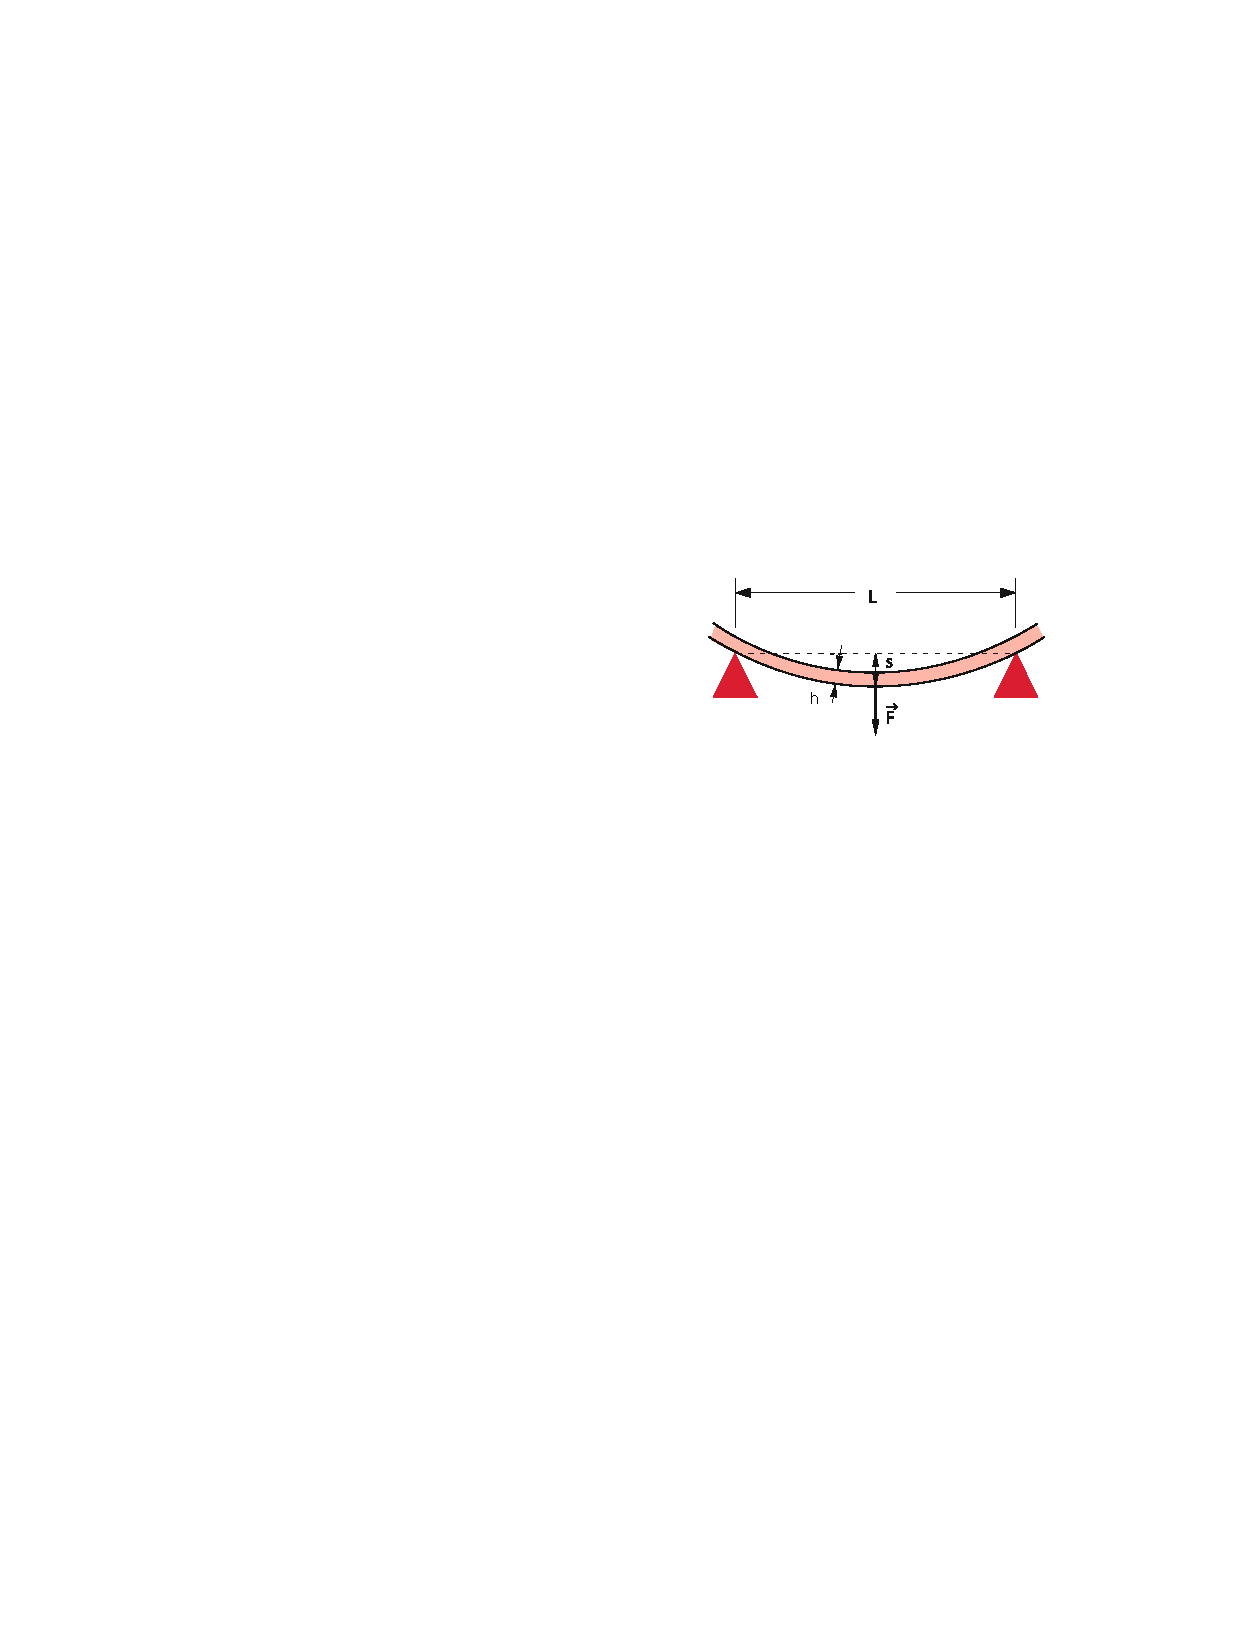
\includegraphics[width=0.8\textwidth]{versuchsaufbau.pdf}}
\renewcommand\thefigure{B2}
\caption[Versuchsaufbau]{Versuchsaufbau \cite{Demtr\"oder}}
\label{Abb:2}
\end{figure}

\subsection{Aufbau}

% describe set up
% insert pic name, designation, toc caption, caption, label
%\halftime{5}{5}{TEXT}{\fbox{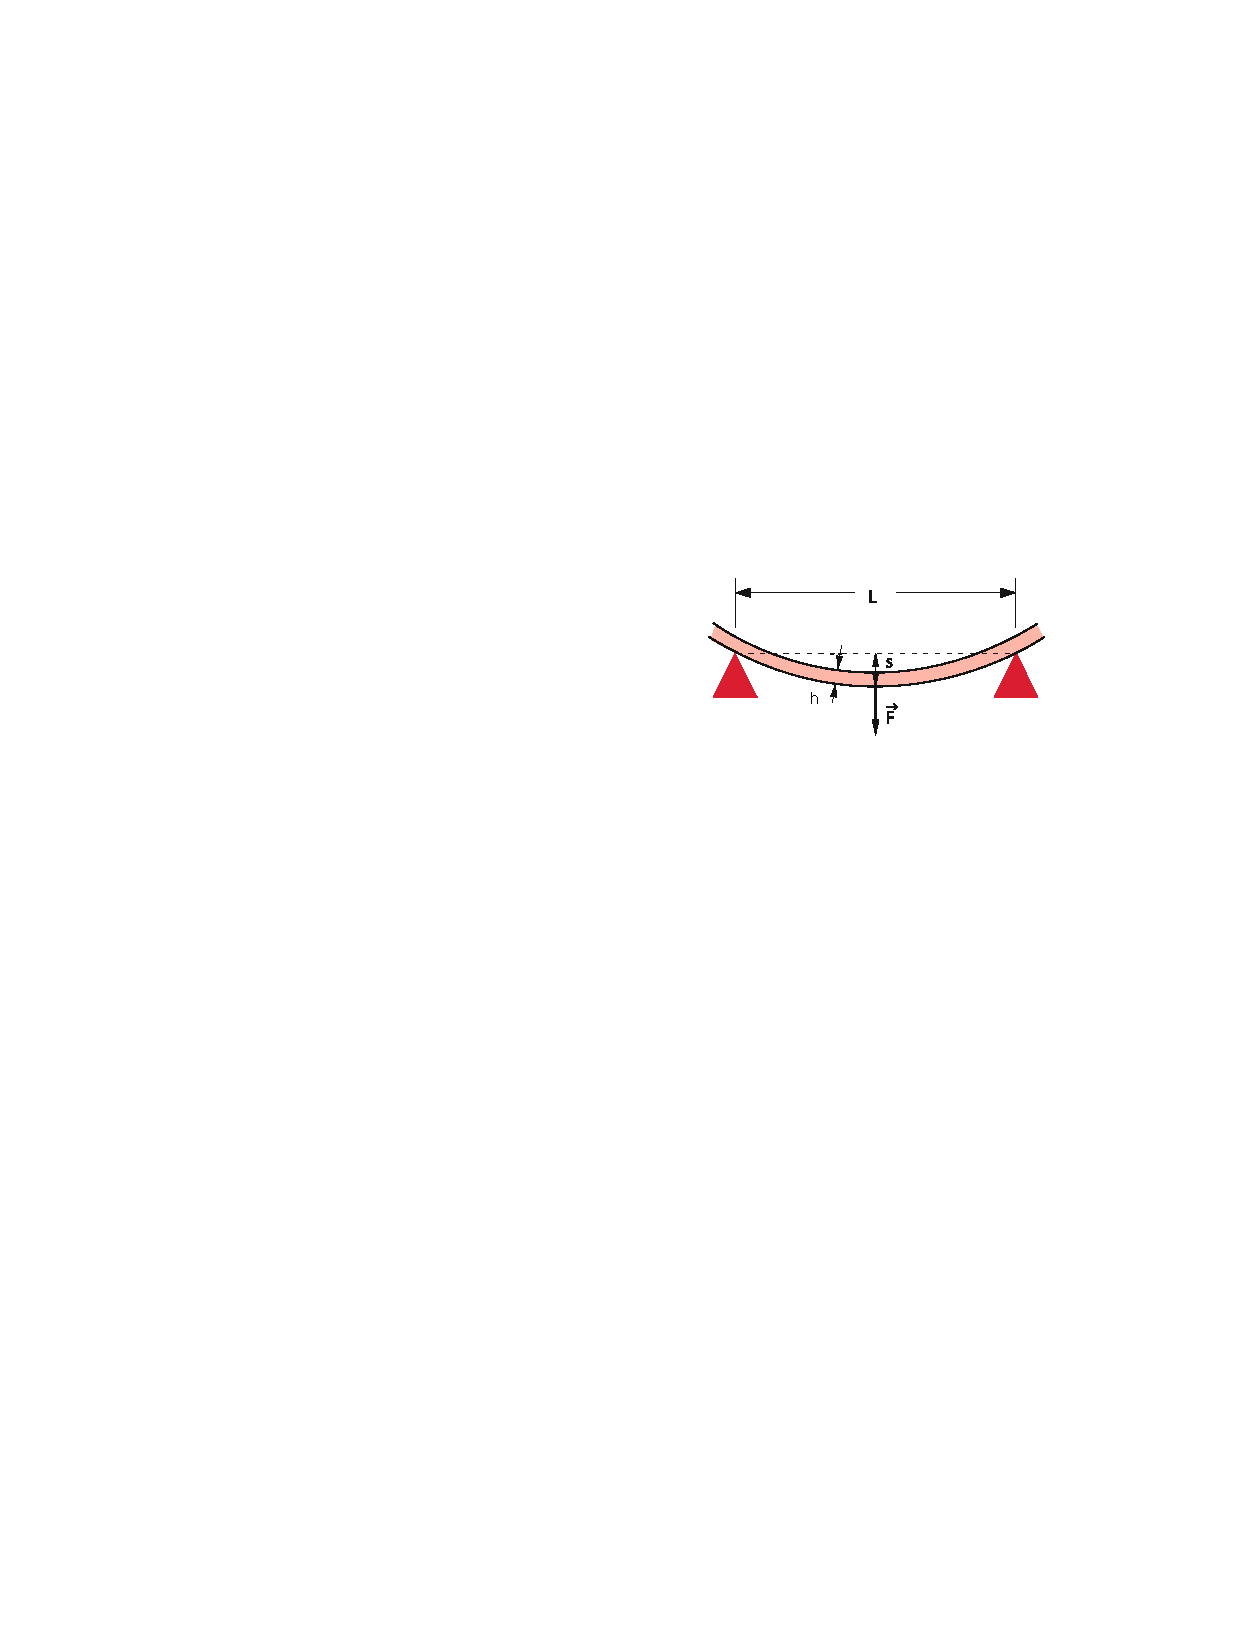
\includegraphics[width=0.8\textwidth]{versuchsaufbau.pdf}}
%   \renewcommand\thefigure{BX}
%\caption[XXXX]{XXXX \cite{Anleitung}}
%\label{Pic:X}}

Vorhanden waren drei St\"abe, jeweils aus Stahl, Aluminium und Messing, welche auf eine optische Bank mit zwei Schneiden platziert werden konnte. An der optischen Bank montiert war ein digitales Messger\"at, welches die Halterung der Gewichte oben ber\"uhrt hat. Um die Ma\ss st\"abe und Gewichte zu messen, waren ein Bandma\ss , eine Messschraube und eine Waage vorhanden. Wie die St\"abe beim Beugen auf den Schneiden lagen kann in Abbildung \ref{Abb:2} betrachtet werden.

\subsection{Durchführung}

% describe exp.
Zu Beginn werden die St\"abe in L\"ange, Breite und H\"ohe gemessen. Da die Messschraube f\"ur die L\"ange zu klein ist, wird sie nur f\"ur Messung der Breite und H\"ohe genutzt. F\"ur die L\"ange muss das Ma\ss band verwendet werden. Am Besten werden alle Messungen mehrmals an verschiedenen Stellen durchgef\"uhrt.

Nachdem alle drei St\"abe ausreichend gemessen wurden, k\"onnen die Gewichte mit der Waage gewogen werden. Um sp\"ater genauer das Gewicht bestimmen zu k\"onnen, kann man jedes Gewicht einzeln messen und mit einem Stift oder Post-its Markierungen setzen, damit das drangewogene Gewicht genauer bestimmt werden kann.

Um die Messung der Biegung durchf\"uhren zu k\"onnen, wird dann ein Stab auf die Schneiden platziert. Man misst zudem noch den Abstand der Auflagefl\"achen. Dies ist sp\"ater die L\"ange, mit der gerechnet wird.

Von dort aus muss zuerst die Linearit\"at \"uberpr\"uft werden. Hierzu werden nacheinander Gewichte drangelegt, sodass man insgesamt f\"ur zehn verschiedenen Gewichten die Biegung hat. Die Biegung wird nach jeder neu drangeh\"angten Masse gemessen und notiert. Hat man die zehn Gewichte drauf, so wird der Vorgang r\"uckw\"arts wiederholt. Diese Messung wird insgesamt zweimal durchgef\"uhrt.

Ist dieser Teil erledigt worden, so misst man als letztes die Durchbiegung gleicherma\ss en f\"ur drei verschiedene Materialien und f\"ur jeweils ein Material zwei verschiedene Ausrichtungen und L\"angen. Hierbei kann man weniger Gewichte insgesamt dranh\"angen. 

\pagebreak

\subsection{Auswertung}

Um die Messwerte anst\"andig darzustellen, k\"onnen wir eine einfache Lineare Regression durchf\"uhren. Da die Werte schon von allein sehr linear verlaufen, werden die Grenzgeraden weggelassen. Dies sind dann wesentlich \"asthetischer aus.

Aufgrund der mehreren Messwerte f\"ur jede Biegung berechnen wir hier mit Mittelwerten. Diese werden mit den folgenden Funktionen berechnet:
\mean
\meanstd

Die f\"ur die lineare Regression ben\"otigten Formeln sind bekannterweise:

\begin{equation}
a=\frac{\sum x_i^2\sum y_i-\sum x_i\sum x_iy_i}{n\sum x_i^2-(\sum x_i)^2}
\end{equation}
\begin{equation}
b=\frac{n\sum x_iy_i-\sum x_i\sum y_i}{n\sum x_i^2-(\sum x_i)^2}
\end{equation}
\begin{equation}
s=\sqrt{\frac{1}{n-2}\sum^n_{i=1}[y_i-(a+bx_i)]^2}
\end{equation}
\begin{equation}
\Delta a=s\sqrt{\frac{\sum x_i^2}{n\sum x_i^2-(\sum x_i)^2}}
\end{equation}
\begin{equation}
\Delta b=s\sqrt{\frac{n}{n\sum x_i^2-(\sum x_i)^2}}
\end{equation}
\pagebreak
Der Graph f\"ur den Vergleich der Materialien sieht dann folgenderma\ss en aus:

\begin{figure}[h]
\centering
\fbox{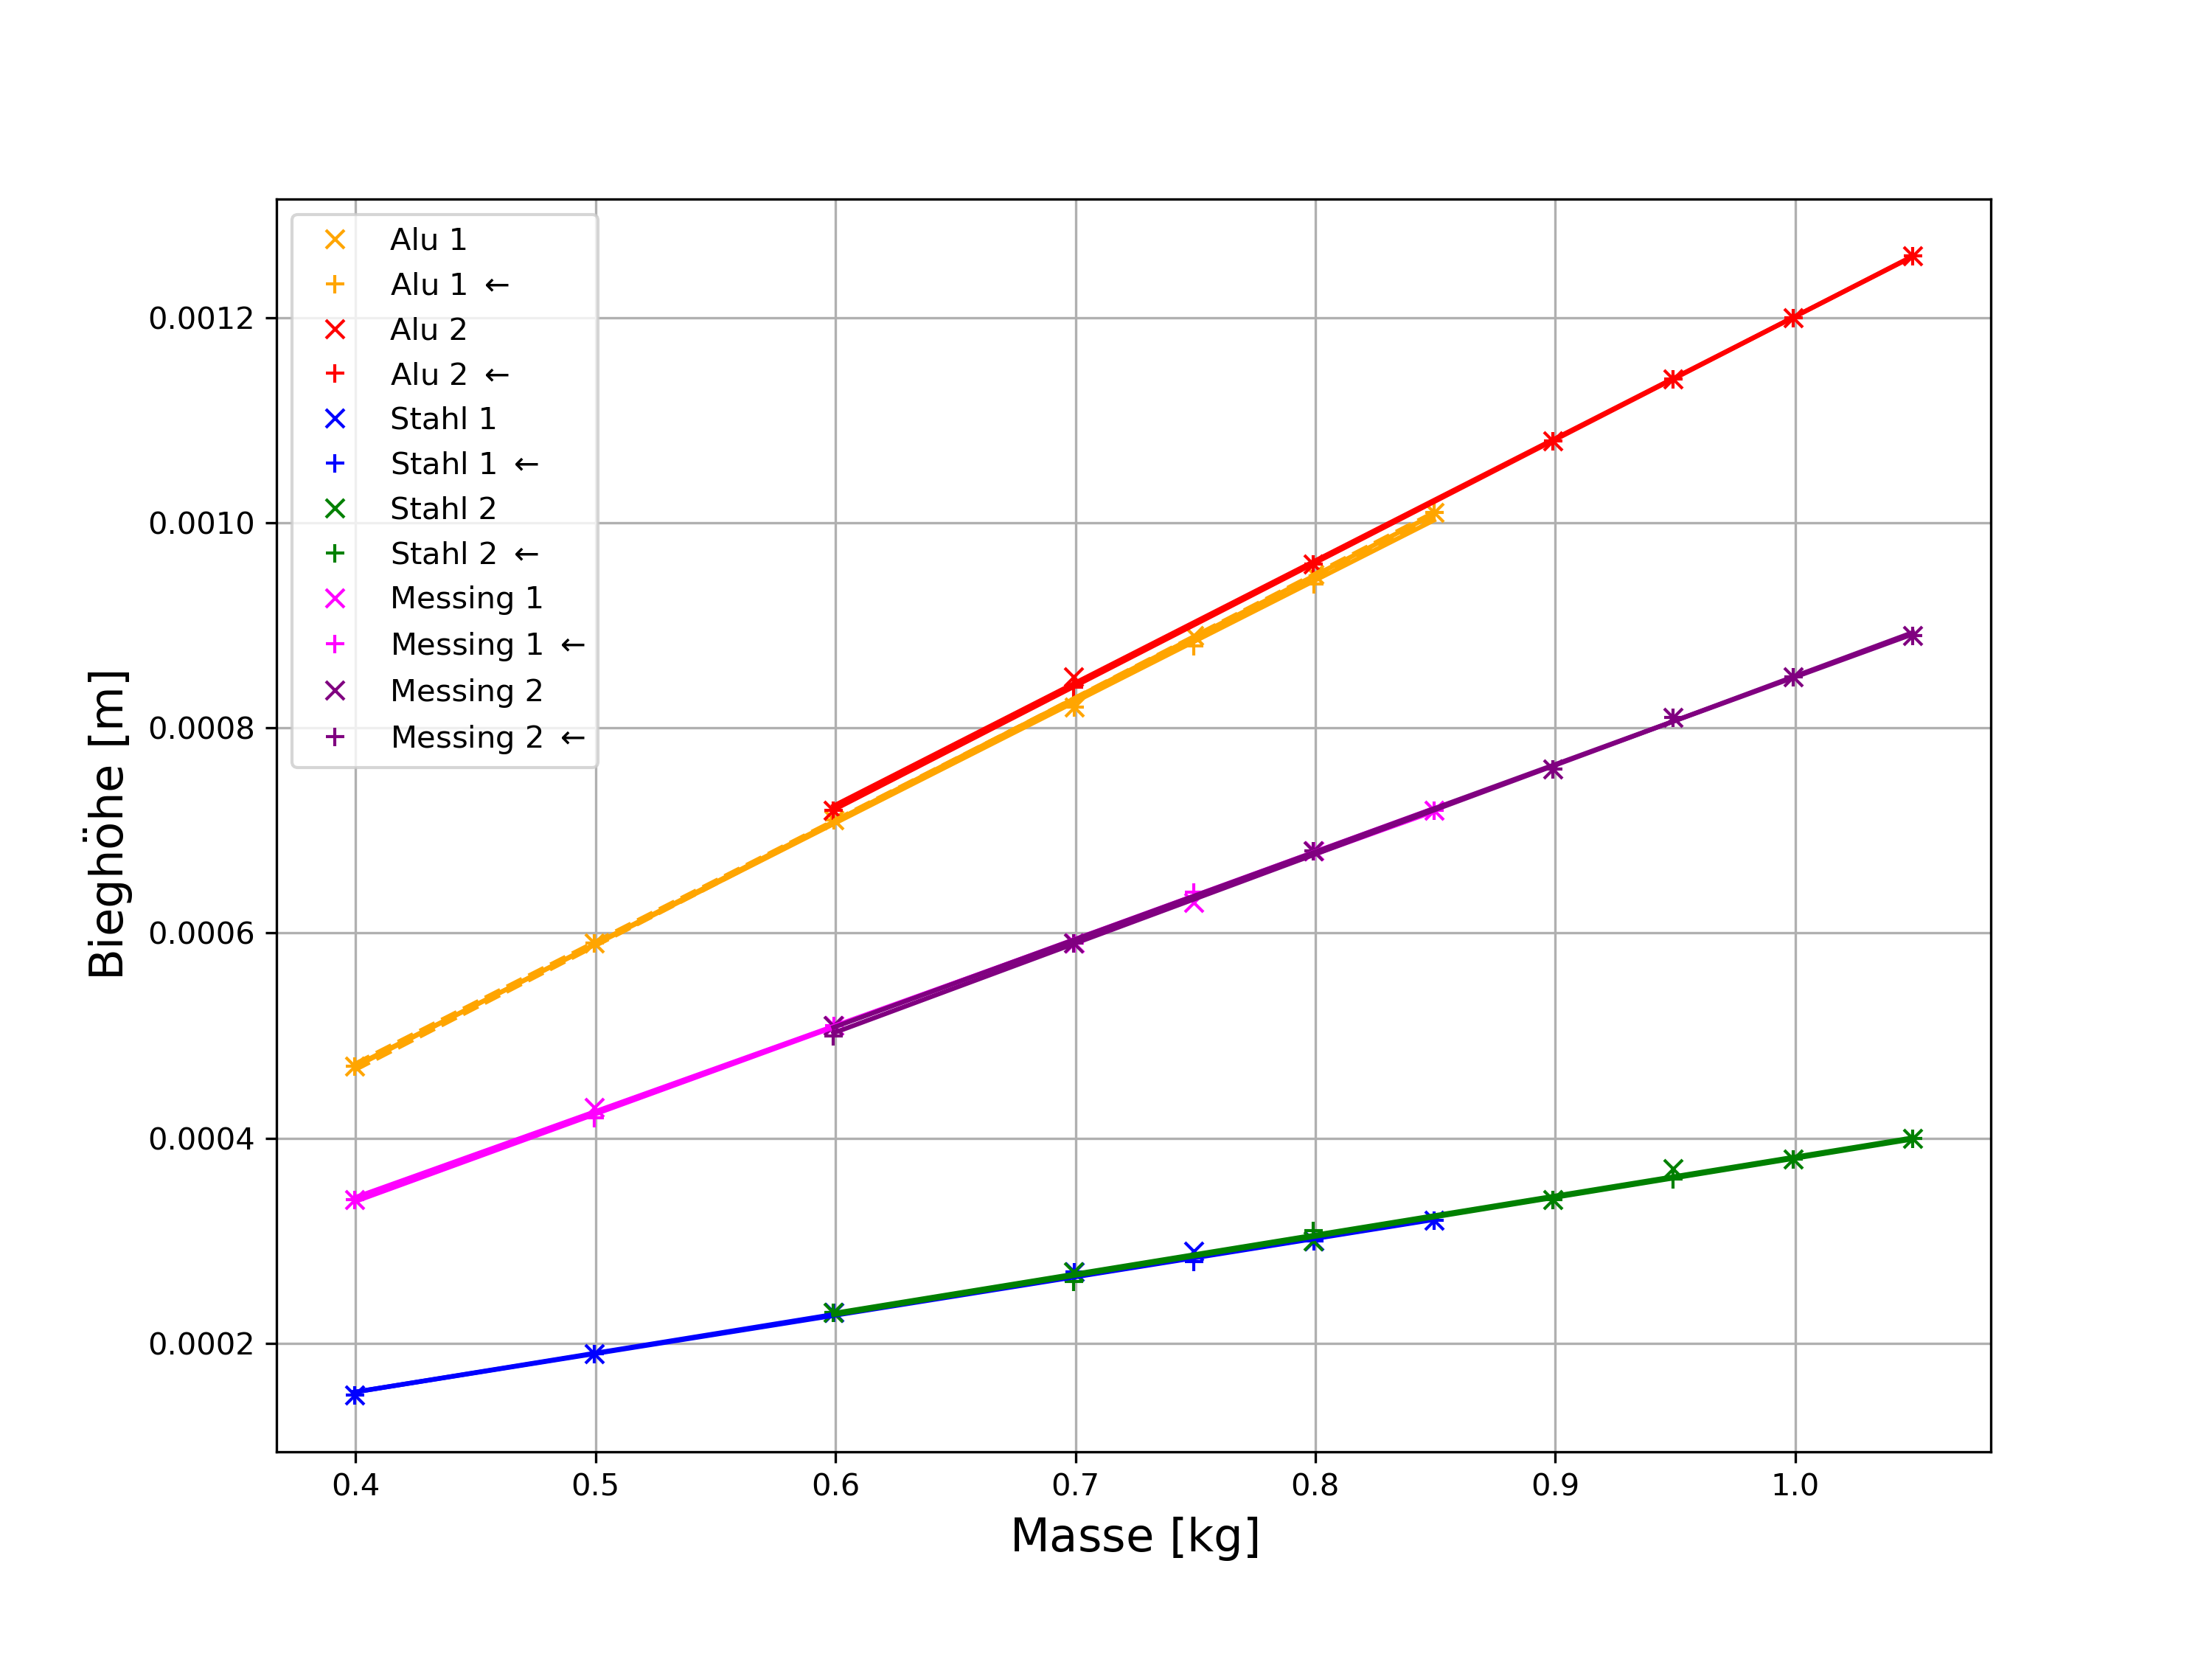
\includegraphics[width=0.8\textwidth]{material.png}}
\renewcommand\thefigure{D1}
\caption[Vergleich der Biegung von Aluminium, Stahl und Messing]{Vergleich der Biegung von Aluminium, Stahl und Messing}
\label{Abb:1}
\end{figure}

Dies wurde bei einem Abstand von $(40.5\pm0.5)$\,cm zwischen den beiden Auflegepunkten f\"ur den Stab durchgef\"uhrt.

\pagebreak

Wieder beim selben Abstand wurde dann auch der Einfluss der \"Anderung der Ausrichtung bei Aluminium \"uberpr\"uft:

\begin{figure}[h]
\centering
\fbox{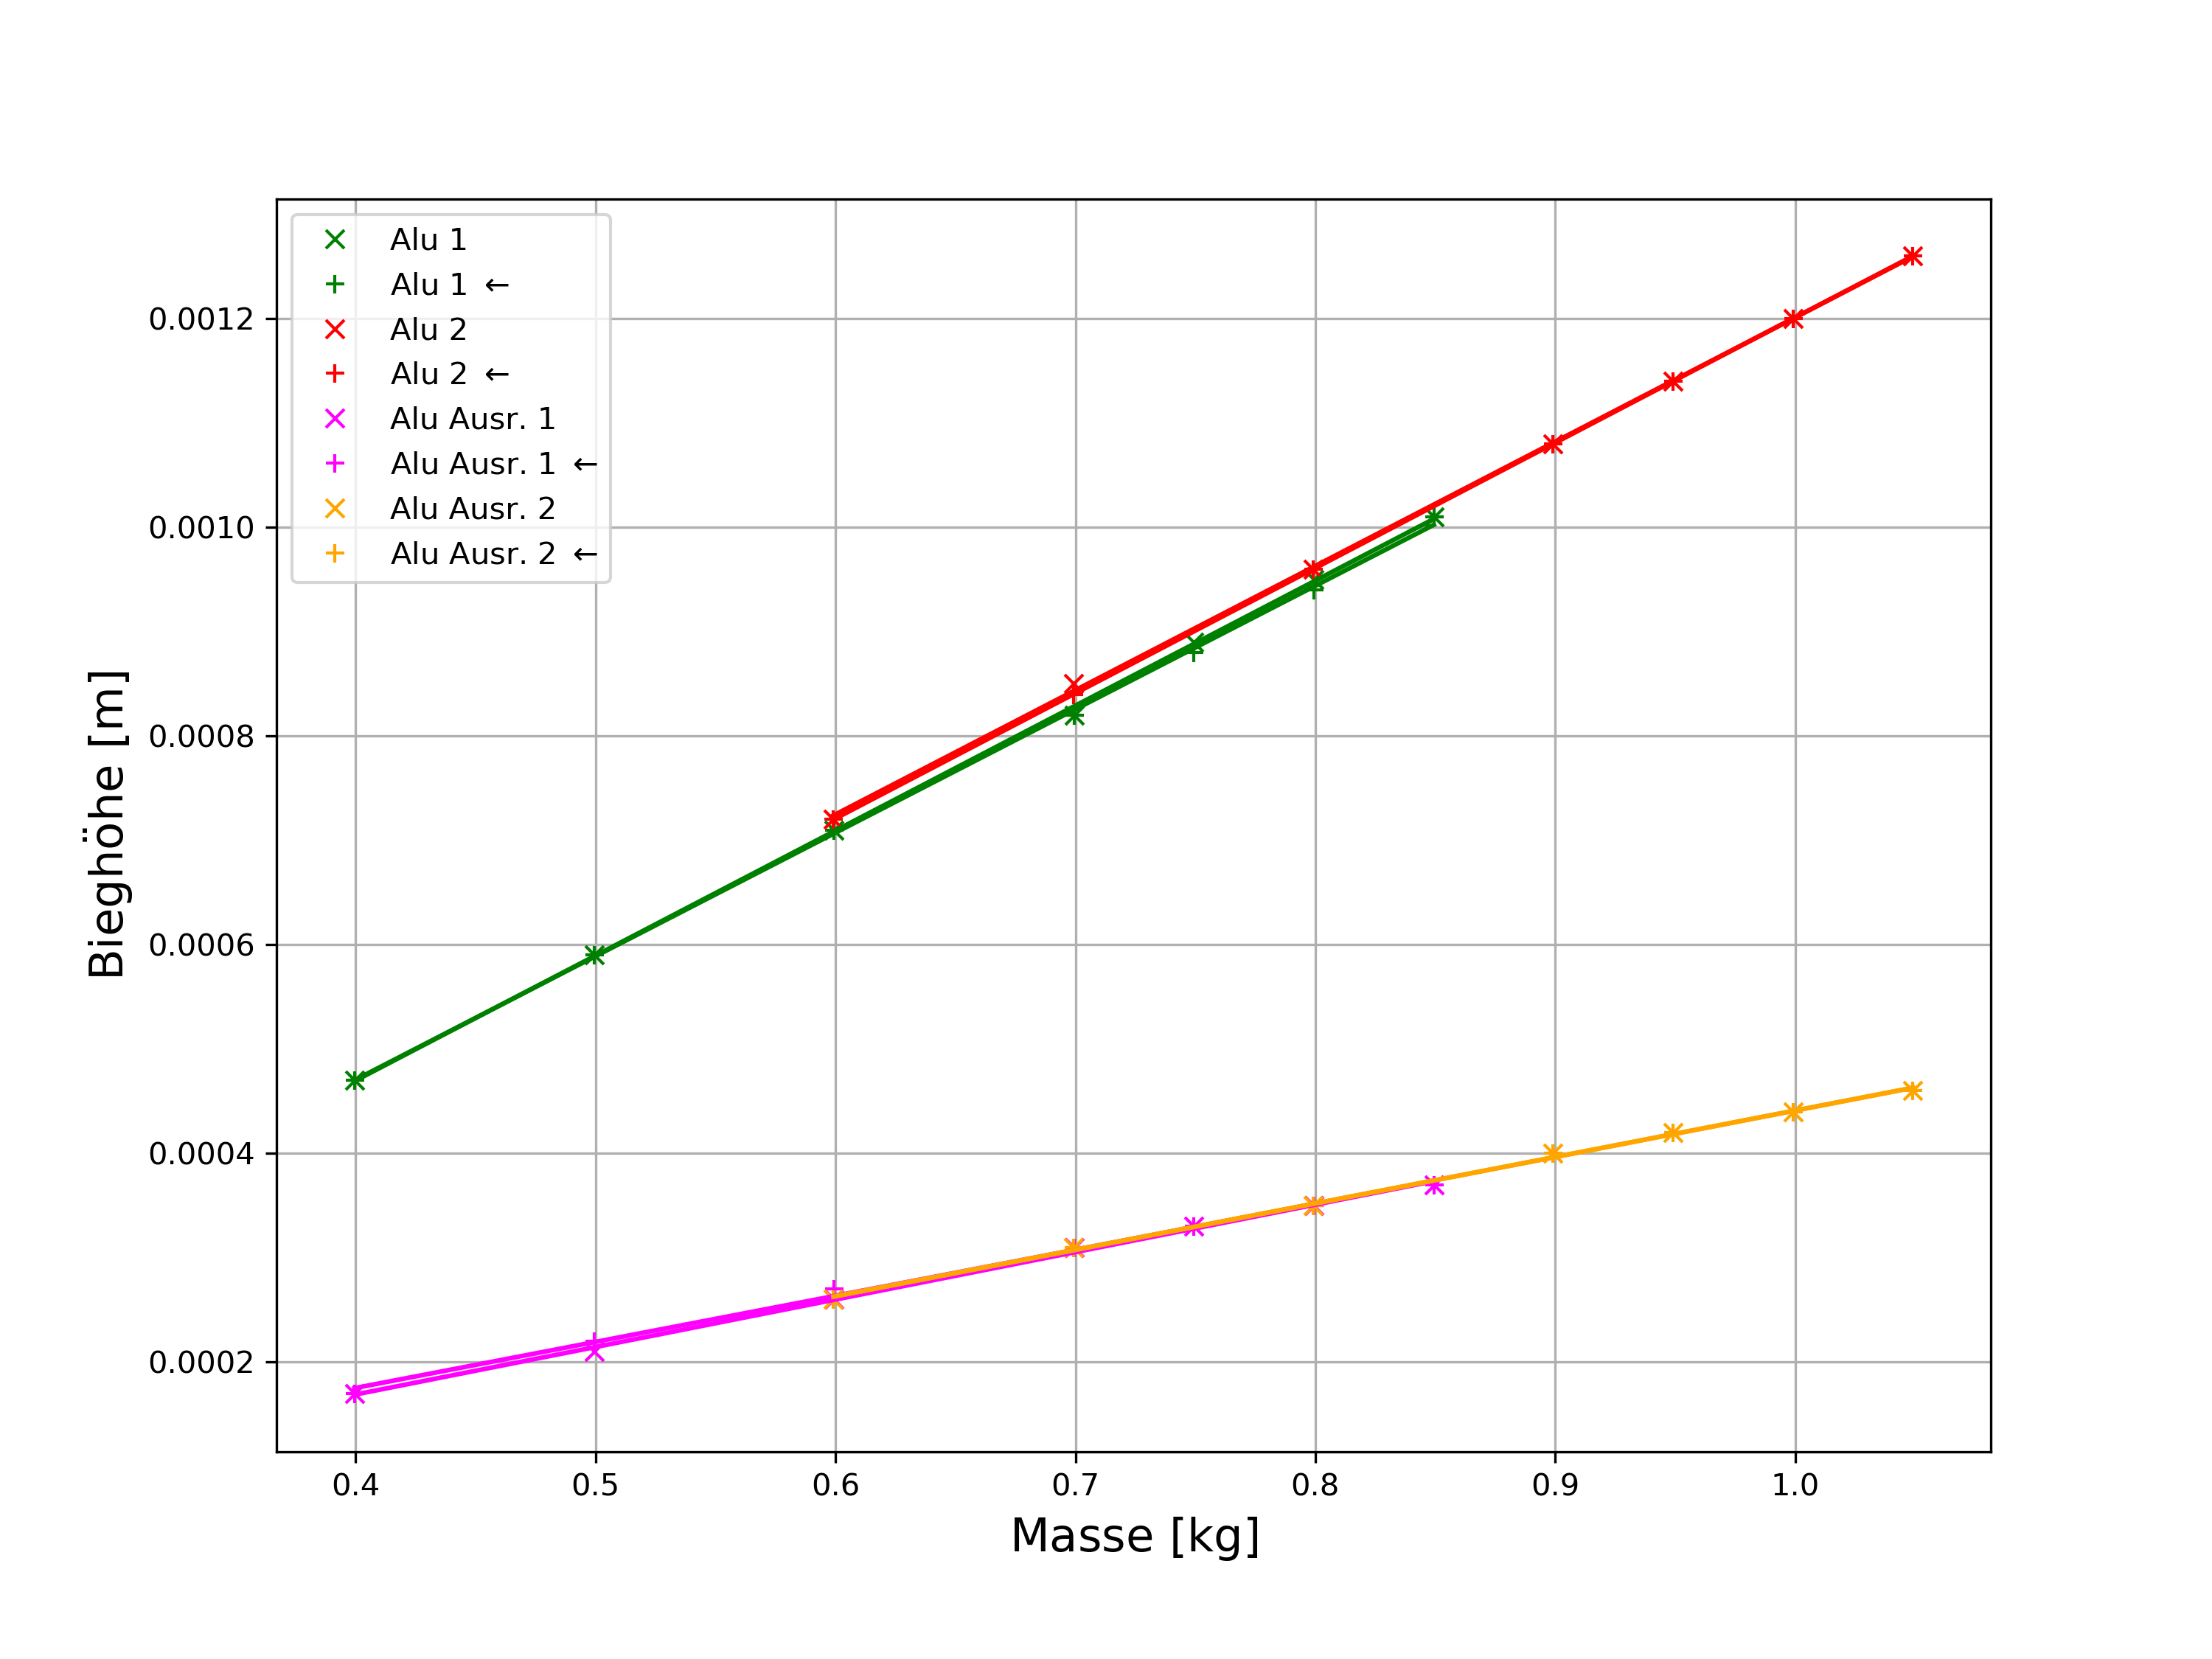
\includegraphics[width=0.8\textwidth]{ausrichtung.png}}
\renewcommand\thefigure{D2}
\caption[Vergleich von Biegung von Aluminium bei verschiedenen Ausrichtungen]{Vergleich von Biegung von Aluminium bei verschiedenen Ausrichtungen}
\label{Abb:2}
\end{figure}

\pagebreak

Als letztes der Vergleich von verschiedenen L\"angen:
\begin{figure}[h]
\centering
\fbox{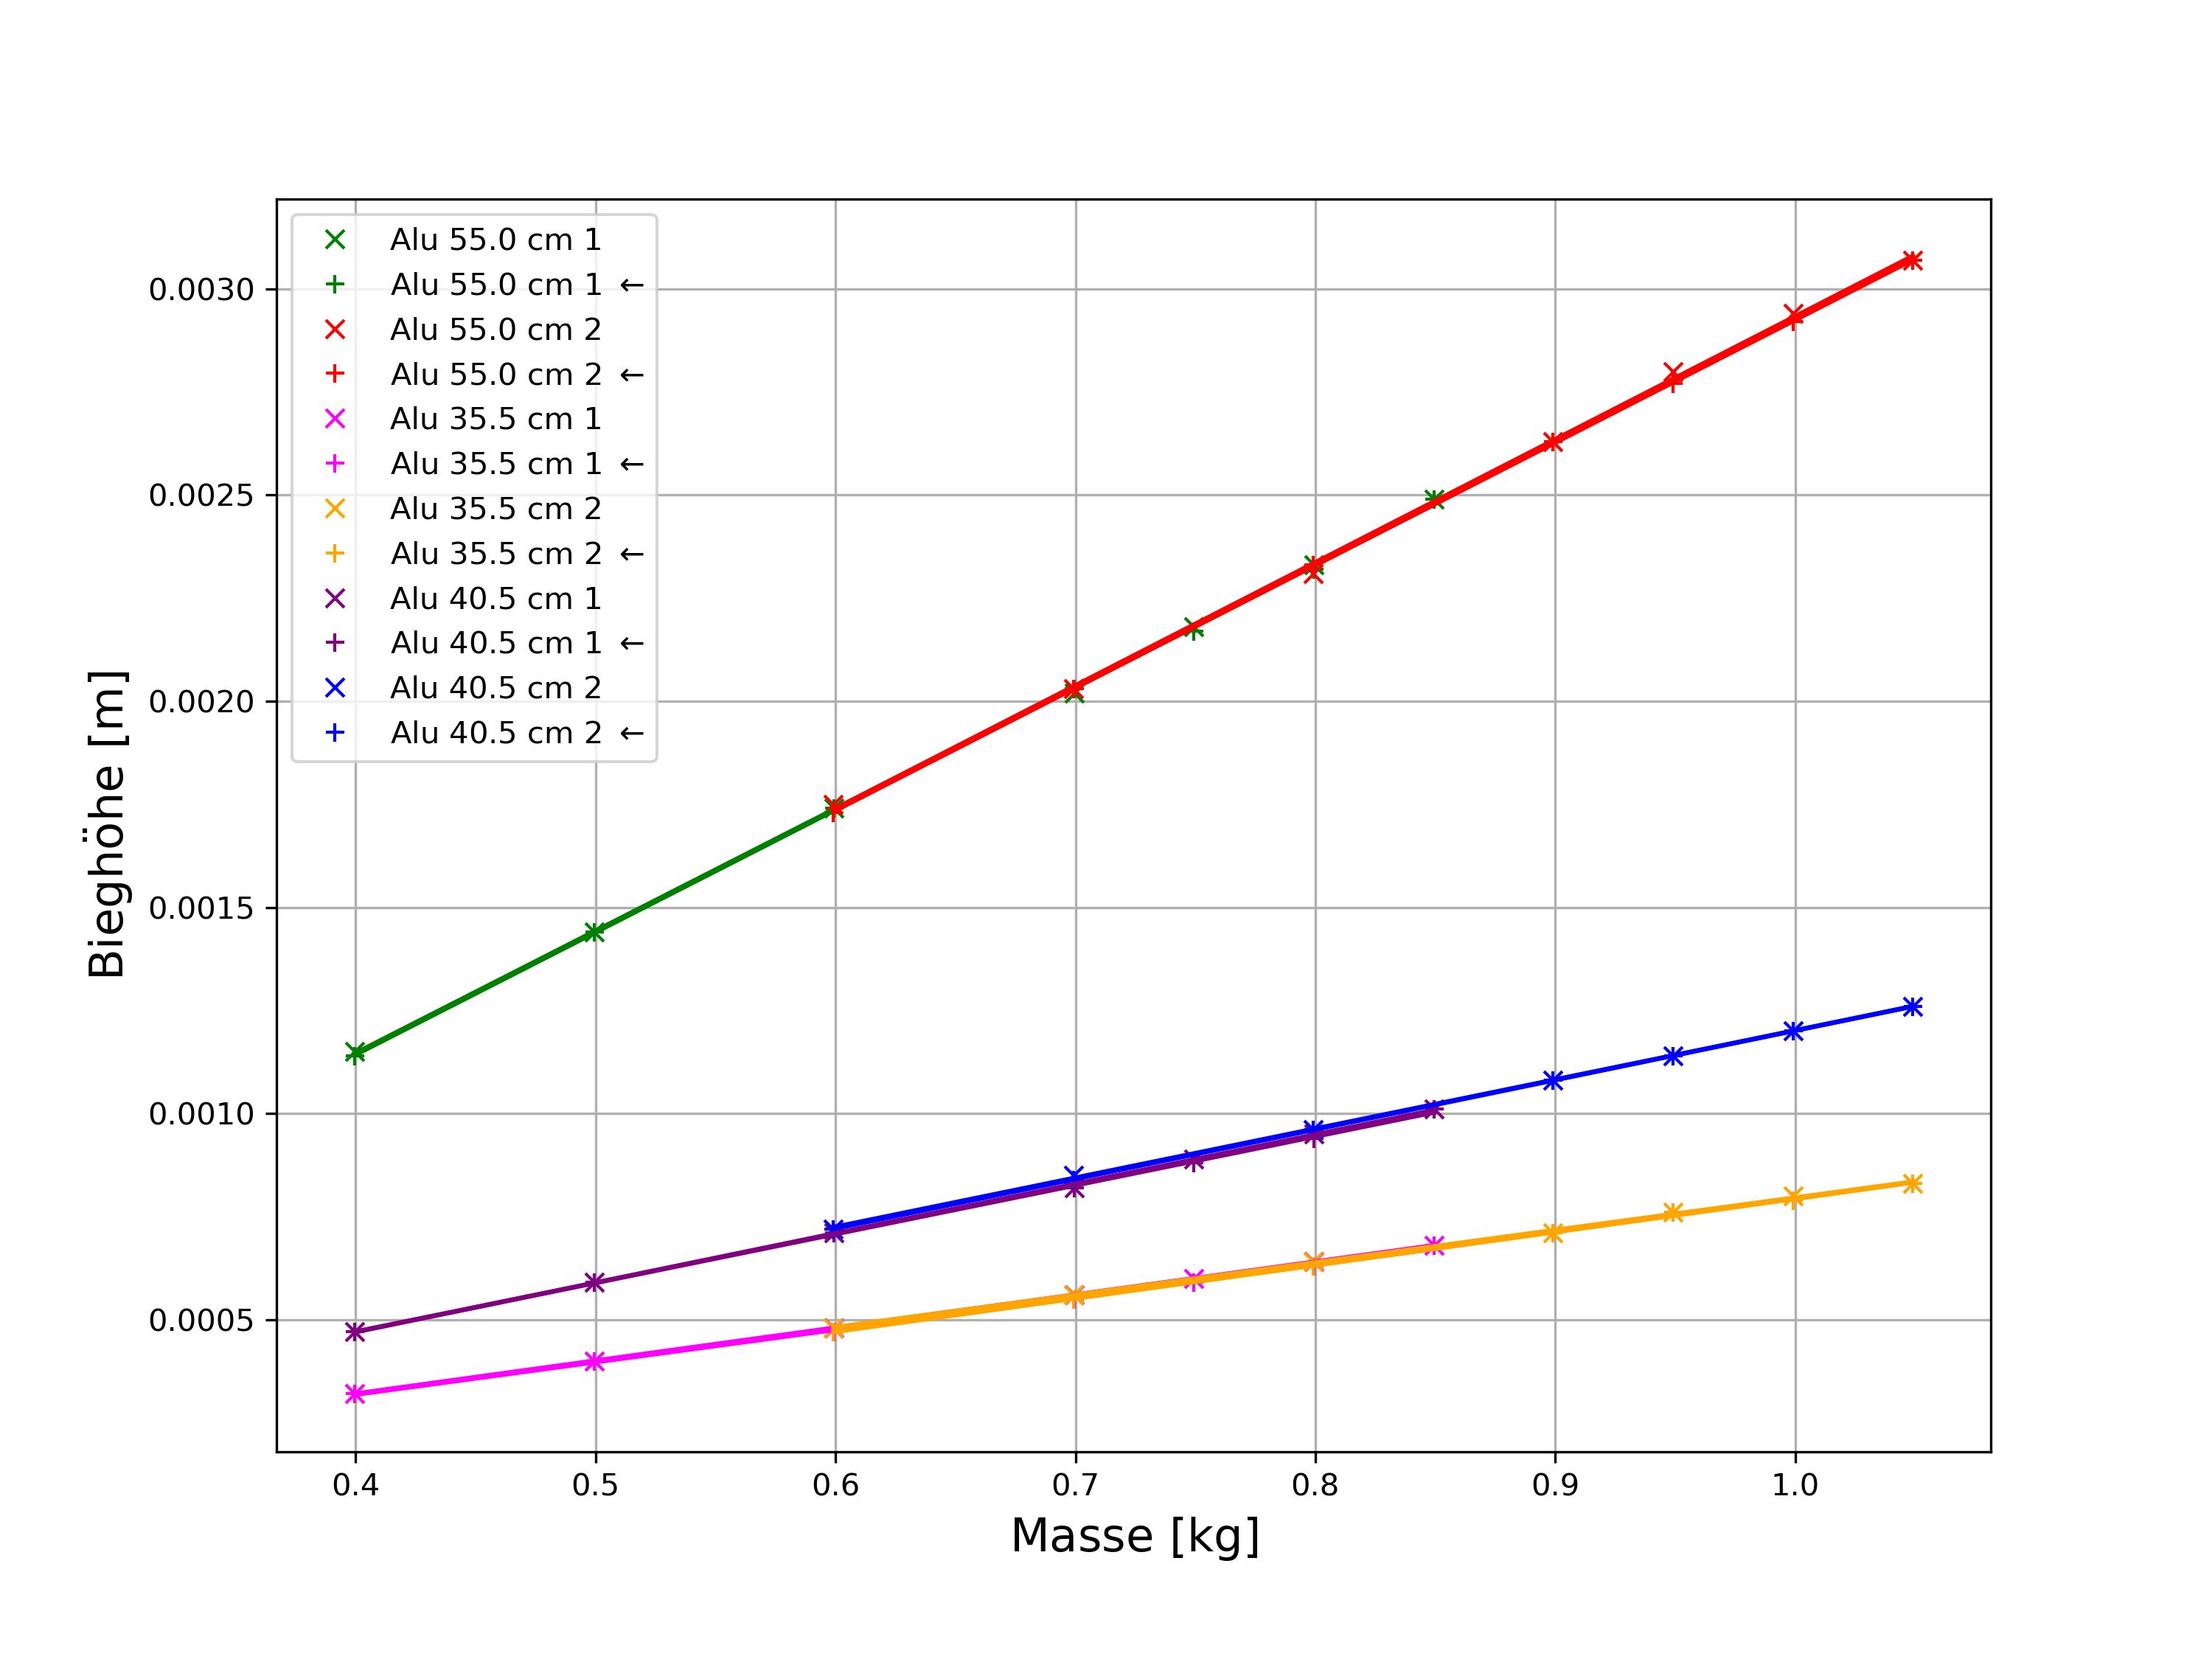
\includegraphics[width=0.8\textwidth]{length.png}}
\renewcommand\thefigure{D3}
\caption[Vergleich von Biegung von Aluminium bei verschiedenen L\"angen]{Vergleich von Biegung von Aluminium bei verschiedenen L\"angen}
\label{Abb:3}
\end{figure}

\pagebreak

Um von hier auf unser Ziel, der Elastizit\"atsmodul, zu kommen, nutzen wir die Formel (\ref{eq:elast}) aus der Theorie. Diese m\"ussen wir jedoch erstmal nach $E$ umstellen. Da wir ja in Abh\"angigkeit von $m$ arbeiten, dr\"ucken wir zuerst unser $F$ als $mg$ aus und lassen dieses $m$ alleine auf der rechten Seite stehen:
\[
E=\frac{l^3g}{s4h^4b}m
\]

Wir ben\"otigen also die L\"ange, Breite und H\"ohe des verwendeten Stabteils, sowie dessen Durchbiegung bei verschiedenen Massen. Wir betrachten erstmal die Formel f\"ur Fehlerrechnung bei Produkten und Quotienten:
\prodquo
Mit unserer Formel dann:
\begin{equation}
\left\vert\frac{\Delta E}{E}\right\vert=\sqrt{\left(3\frac{\Delta l}{l}\right)^2+\left(-\frac{\Delta s}{s}\right)^2+\left(-4\frac{\Delta h}{h}\right)^2+\left(-\frac{\Delta b}{b}\right)^2}
\end{equation}

Da die Unsicherheit der Steigung klein ist und nur das 1-Fache dessen in die Unsicherheit von $E$ eingeht, ist diese zu vernachl\"assigen. Die Unsicherheit von $b$ k\"onnen wir auch vernachl\"assigen.


Wir nutzen also unsere Steigung aus der linearen Regression als $s$ und rechnen hiermit als Werte f\"ur $E$:

\begin{table}[h]
\centering
\caption{Berechnete Werte f\"ur $E$} \vspace{11pt}
$\begin{array}{l}
\textrm{Unsicherheiten:}\\
\textrm{L\"ange: } \pm 0.005\,\textrm{cm}\\
\end{array}$
\begin{tabular}{ccc}
\toprule
\textrm{Messreihe} & \textrm{L\"ange}\,[\textrm{cm}] & \textrm{Elastizit\"atsmodul}\,$\left[\nicefrac{\mathrm{N}}{\mathrm{m^2}}\right]$ \\
\midrule 
\textrm{Aluminium} & 40.5 & $(6.75\pm0.025)\times10^{10}$ \\
\textrm{Stahl} & 40.5 & $(2.137\pm0.008)\times10^{11}$ \\
\textrm{Messing} & 40.5 & $(9.49\pm0.035)\times10^{10}$ \\
\hline
\textrm{Alu umgedreht} & 40.5 & $(6.46\pm0.024)\times10^{10}$ \\
\textrm{Aluminium} & 55.0 & $(6.78\pm0.018)\times10^{10}$ \\ 
\textrm{Aluminium} & 33.5 & $(5.74\pm0.026)\times10^{10}$ \\ 
\textrm{Alu 10 Messungen} & 40.5 & $(6.76\pm0.025)\times10^{10}$ \\ 
\bottomrule
\end{tabular}
\phantom{$\begin{array}{l}
\textrm{Unsicherheiten:}\\
\textrm{XXXX: } \pm XX \textrm{XX}\\
\end{array}$}
\label{Tab:1}
\end{table}

Die genauen Werte f\"ur die Breite und H\"ohe der St\"abe sind im Anhang zu finden. Wir verwenden als Wert f\"ur $g$ $9.81\,\nicefrac{\mathrm{m}}{\mathrm{s}^2}$.

\pagebreak

\section{Diskussion}

Die entsprechenden Literaturwerte lauten \cite{Anleitung}:

\begin{itemize}
\item Aluminium: $E=(69\ldots72.5)\times10^3\,\nicefrac{\mathrm{N}}{\mathrm{mm^2}}$
\item Stahl: $E=(195\ldots210)\times10^3\,\nicefrac{\mathrm{N}}{\mathrm{mm^2}}$
\item Messing: $E=(90\ldots95)\times10^3\,\nicefrac{\mathrm{N}}{\mathrm{mm^2}}$
\end{itemize}

Um die Vertr\"aglichkeit unserer Werte zu \"uberpr\"ufen betrachten wir die 2-$\sigma$ Bereiche unserer gemessenen Werte:

\begin{table}[h]
\centering
\caption{Berechnete Werte f\"ur $E$} \vspace{11pt}
$\begin{array}{l}
\textrm{Unsicherheiten:}\\
\textrm{L\"ange: } \pm 0.005\,\textrm{cm}\\
\end{array}$
\begin{tabular}{ccc}
\toprule
\textrm{Messreihe} & \textrm{L\"ange}\,[\textrm{cm}] & \textrm{2-}$\sigma$\textrm{ Bereich von }$E$\,$\left[\nicefrac{\mathrm{N}}{\mathrm{m^2}}\right]$ \\
\midrule 
\textrm{Aluminium} & 40.5 & $(6.75\pm0.050)\times10^{10}$ \\
\textrm{Stahl} & 40.5 & $(2.137\pm0.016)\times10^{11}$ \\
\textrm{Messing} & 40.5 & $(9.49\pm0.070)\times10^{10}$ \\
\hline
\textrm{Alu umgedreht} & 40.5 & $(6.46\pm0.048)\times10^{10}$ \\
\textrm{Aluminium} & 55.0 & $(6.78\pm0.036)\times10^{10}$ \\ 
\textrm{Aluminium} & 33.5 & $(5.74\pm0.052)\times10^{10}$ \\ 
\textrm{Alu 10 Messungen} & 40.5 & $(6.76\pm0.050)\times10^{10}$ \\ 
\bottomrule
\end{tabular}
\phantom{$\begin{array}{l}
\textrm{Unsicherheiten:}\\
\textrm{XXXX: } \pm XX \textrm{XX}\\
\end{array}$}
\label{Tab:1}
\end{table}

Wir k\"onnen klar erkennen, dass f\"ur Aluminium keine Messung im 2-$\sigma$ Bereich mit den Literaturwerten \"ubereinstimmt. Alle liegen unterhalb des Wertebereichs. Am auff\"alligsten ist hier die Messung bei einer L\"ange von 33.5\,cm, da dieser deutlich am weitesten entfernt ist.

Unsere Messungen f\"ur Stahl und Messing stimmen jedoch \"uberein. Interessant ist hier aber, dass beide an der oberen Grenze des Bereichs vom Literaturwert liegen.

Die Ursache hiervon ist vermutlich ein zu fein gesch\"atzter Fehler des f\"ur die L\"angenmessung genutzten Bandma\ss es. Verdoppeln wir diesen Fehler, so verdoppeln sich auch die Fehler unserer Endergebnisse. Vergleichen wir die Werte nach dieser Verdopplung, so liegt nur noch die Messung von Aluminium bei 33.5\,cm au\ss erhalb des 2-$\sigma$ Bereichs. In diesem Fall w\"aren alle anderen Messwerte mit den Literaturwerten vertr\"aglich.

Jedoch muss man sich immer noch fragen, weshalb die Werte von Messing und Stahl an der oberen und die von Aluminium an der unteren Grenze des Wertebereichs liegen. Offensichtlich haben andere Fehler noch einen Einfluss.

Erstmal klar ist, dass noch zus\"atzliche Kr\"afte wirken, welche durch das Eigengewicht der St\"abe, das Gewicht der Halterung und der Andruckkraft des Messger\"ats ausge\"ubt werden. Da dieser Versuch sich aber im Proportionalit\"atsbereich aufh\"alt, m\"ussen diese Kr\"afte nicht ber\"ucksichtigt werden, da sie nur den Nullpunkt des Messger\"ats verschieben. Dies ist also vermutlich nicht die Ursache.

Suchen wir nach anderen Fehlern, so muss zuerst die Form der Literaturwerte klarifiziert werden; Stahl-, Aluminium- und Messingst\"abe werden je nach Werkstoffzusammensetzung andere Elastizit\"atsmodule haben. Wir k\"onnen also davon ausgehen, dass die St\"abe in diesen Wertebereichen ihre Elastizit\"atsmodule haben und nicht aufgrund von unreiner Zusammensetzung als systematischer Fehler gelten k\"onnen.

Die n\"achste Fehlerquelle, die wie betrachten werden, ist die, dass die Halterungen der St\"abe m\"oglicherweise Bewegungsanf\"allig waren, wodurch die L\"angen noch ungenauer werden w\"urden. Gleicherma\ss en k\"onnten die St\"abe auch nicht gerade auf den Halterungen stehen. H\"atte das Ger\"at bessere Halterungen, bei denen die St\"abe immer zentriert w\"aren und keine Bewegung m\"oglich ist, so w\"aren eventuell bessere Ergebnisse m\"oglich.

Betrachten wir nochmal unsere Gleichung f\"ur $E$:
\[
E=\frac{l^3g}{s4h^4b}m
\]
Klar ist, dass $g$ keinen gr\"o\ss eren Einfluss hat und auch schon relativ genau gew\"ahlt wurde. Au\ss erdem wurden die Massen der einzelnen Gewichte vor der Messung alle gemessen und Markierungen gesetzt, wodurch wir ein Problem mit den Massen ausschlie\ss en k\"onnen. Uns bleiben also noch Fehler auf $s$, $h$ und $b$. Da f\"ur die Messung der Breite und H\"ohe eine Messschraube genutzt wurde, ist ein Problem hier eher unwahrscheinlich. Vermutlich k\"onnte also unser Fehler auch bei dem digitalen Messger\"at liegen.

\vfill

\begin{thebibliography}{9}
%\bibitem{Uncertainties}''Correlations between variables are automatically handled, which sets this module apart from many existing error propagation codes.'' - \url{https://pythonhosted.org/uncertainties/}
\bibitem{Anleitung} Physikalisches Institut der Albert-Ludwigs-Universität Freiburg (Hrsg.) (08/2018): Versuchsanleitungen zum Physiklabor für Anfänger*innen, Teil 1, Ferienpraktikum im Sommersemester 2018.
\bibitem{Demtr\"oder} Demtr\"oder, Experimentalphysik 1, \url{https://www.springer.com/us/book/9783662464151}, Kapitel 6.2.4
\end{thebibliography}

%\pagebreak

%\section{Anhang: Messwerte}

%\begin{table}[h]
%\centering
%\caption{XXXX} \vspace{11pt}
%$\begin{array}{l}
%\textrm{Unsicherheiten:}\\
%\textrm{XXXX: } \pm XX \textrm{XX}\\
%\end{array}$
%\begin{tabular}{ccc}
%\toprule
%\textrm{XXXX}/\textrm{XX} & \textrm{XXXX}/\textrm{XX} & \textrm{XXXX}/\textrm{XX} \\
%\midrule 
%2 & 0.26 & 0.23\\
%\hline
%4 & 0.33 & 0.25\\
%\hline 
%5 & & 0.3\\
%\hline 
%6 & 1.25 & 0.83\\
%\hline 
%8 & 3.9 & 0.83\\ 
%\hline
%9 & 4.75 & 4.6\\ 
%\hline
%10 & 4.7 &\\ 
%\bottomrule
%\end{tabular}
%\phantom{$\begin{array}{l}
%\textrm{Unsicherheiten:}\\
%\textrm{XXXX: } \pm XX \textrm{XX}\\
%\end{array}$}
%\label{Tab:X}
%\end{table}

%\begin{figure}[p]
%\centering
%\fbox{\includegraphics[width=0.8\textwidth]{NAME}}
%\renewcommand\thefigure{BX}
%\caption[XXXX]{XXXX}
%\label{Abb:X}
%\end{figure}
\end{document}